\documentclass[tikz]{standalone}
\usepackage{tikz}
\usetikzlibrary{arrows.meta,positioning,shapes.geometric,shapes.misc,fit,backgrounds,calc,decorations.pathreplacing}

\definecolor{cBuilder}{HTML}{3D5A80}
\definecolor{cDocumenter}{HTML}{C07C38}
\definecolor{cVerifier}{HTML}{A04050}
\definecolor{cCoordinator}{HTML}{6B5CA5}
\definecolor{cMonitor}{HTML}{488B49}
\definecolor{cEmpirical}{HTML}{2B7A78}

\begin{document}
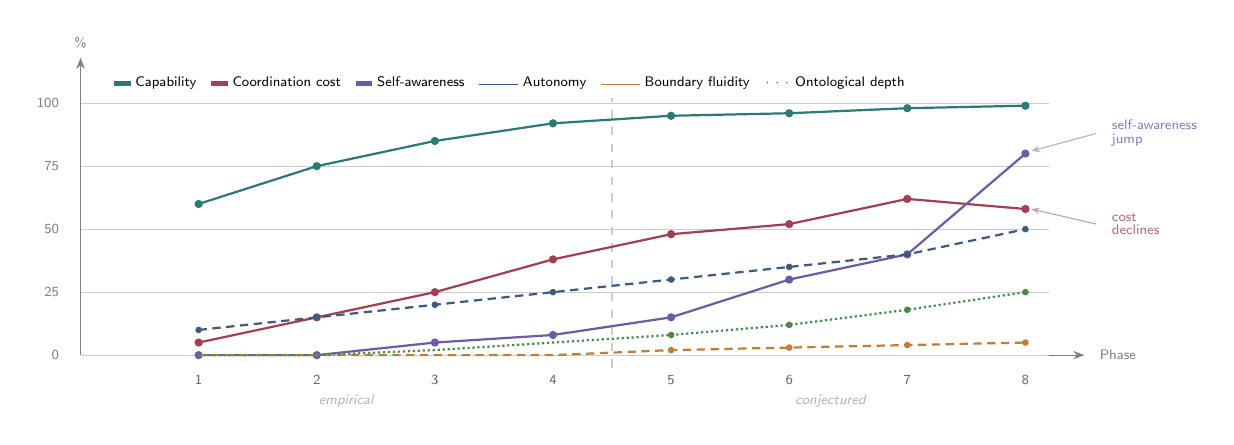
\begin{tikzpicture}[x=1.5cm, y=3.2cm]
% Axes
\draw[-{Stealth[length=4pt]}, black!50] (0,0) -- (8.5,0) node[right, font=\tiny\sffamily, xshift=2pt] {Phase};
\draw[-{Stealth[length=4pt]}, black!50] (0,0) -- (0,1.18) node[above, font=\tiny\sffamily] {\%};

% Y-axis ticks
\foreach \y/\l in {0/0, 0.25/25, 0.5/50, 0.75/75, 1.0/100} {
    \draw[black!20] (0,\y) -- (8.2,\y);
    \node[left, font=\tiny\sffamily, text=black!50] at (-0.1,\y) {\l};
}

% X-axis labels
\foreach \x/\l in {1/1, 2/2, 3/3, 4/4, 5/5, 6/6, 7/7, 8/8} {
    \node[below, font=\tiny\sffamily, text=black!60] at (\x,-0.04) {\l};
}

% Empirical / conjectured boundary - subtle, no text in data area
\draw[dashed, black!20, thin] (4.5,-0.05) -- (4.5,1.02);
\node[font=\tiny\sffamily\itshape, text=black!30, anchor=north] at (2.25,-0.12) {empirical};
\node[font=\tiny\sffamily\itshape, text=black!30, anchor=north] at (6.35,-0.12) {conjectured};

% Data: Capability (teal)
\draw[cEmpirical, thick] plot coordinates {(1,0.60) (2,0.75) (3,0.85) (4,0.92) (5,0.95) (6,0.96) (7,0.98) (8,0.99)};
\foreach \x/\y in {1/0.60, 2/0.75, 3/0.85, 4/0.92, 5/0.95, 6/0.96, 7/0.98, 8/0.99} {
    \fill[cEmpirical] (\x,\y) circle (1.5pt);
}

% Data: Coordination cost (red)
\draw[cVerifier, thick] plot coordinates {(1,0.05) (2,0.15) (3,0.25) (4,0.38) (5,0.48) (6,0.52) (7,0.62) (8,0.58)};
\foreach \x/\y in {1/0.05, 2/0.15, 3/0.25, 4/0.38, 5/0.48, 6/0.52, 7/0.62, 8/0.58} {
    \fill[cVerifier] (\x,\y) circle (1.5pt);
}

% Data: Self-awareness (purple)
\draw[cCoordinator, thick] plot coordinates {(1,0.00) (2,0.00) (3,0.05) (4,0.08) (5,0.15) (6,0.30) (7,0.40) (8,0.80)};
\foreach \x/\y in {1/0.00, 2/0.00, 3/0.05, 4/0.08, 5/0.15, 6/0.30, 7/0.40, 8/0.80} {
    \fill[cCoordinator] (\x,\y) circle (1.5pt);
}

% Data: Boundary fluidity (orange)
\draw[cDocumenter, thick, densely dashed] plot coordinates {(1,0.00) (2,0.00) (3,0.00) (4,0.00) (5,0.02) (6,0.03) (7,0.04) (8,0.05)};
\foreach \x/\y in {5/0.02, 6/0.03, 7/0.04, 8/0.05} {
    \fill[cDocumenter] (\x,\y) circle (1.2pt);
}

% Data: Autonomy (blue)
\draw[cBuilder, thick, densely dashed] plot coordinates {(1,0.10) (2,0.15) (3,0.20) (4,0.25) (5,0.30) (6,0.35) (7,0.40) (8,0.50)};
\foreach \x/\y in {1/0.10, 2/0.15, 3/0.20, 4/0.25, 5/0.30, 6/0.35, 7/0.40, 8/0.50} {
    \fill[cBuilder] (\x,\y) circle (1.2pt);
}

% Data: Ontological depth (pink/monitor green)
\draw[cMonitor, thick, densely dotted] plot coordinates {(1,0.00) (2,0.00) (3,0.02) (4,0.05) (5,0.08) (6,0.12) (7,0.18) (8,0.25)};
\foreach \x/\y in {5/0.08, 6/0.12, 7/0.18, 8/0.25} {
    \fill[cMonitor] (\x,\y) circle (1.2pt);
}

% Legend
\node[font=\tiny\sffamily, anchor=west] at (0.2,1.08) {%
    \textcolor{cEmpirical}{\rule{6pt}{2pt}} Capability\quad
    \textcolor{cVerifier}{\rule{6pt}{2pt}} Coordination cost\quad
    \textcolor{cCoordinator}{\rule{6pt}{2pt}} Self-awareness\quad
    \textcolor{cBuilder}{\rule[0.3ex]{6pt}{0.4pt}\rule[0.3ex]{2pt}{0.4pt}\rule[0.3ex]{6pt}{0.4pt}} Autonomy\quad
    \textcolor{cDocumenter}{\rule[0.3ex]{6pt}{0.4pt}\rule[0.3ex]{2pt}{0.4pt}\rule[0.3ex]{6pt}{0.4pt}} Boundary fluidity\quad
    \textcolor{cMonitor}{$\cdots$} Ontological depth
};

% Annotations - right margin, outside plot area
\draw[-{Stealth[length=3pt]}, cCoordinator!50, thin] (8.6,0.88) -- (8.05,0.81);
\node[font=\tiny\sffamily, text=cCoordinator!80, anchor=west, align=left] at (8.65,0.88) {self-awareness\\[-1pt]jump};

\draw[-{Stealth[length=3pt]}, cVerifier!50, thin] (8.6,0.52) -- (8.05,0.58);
\node[font=\tiny\sffamily, text=cVerifier!80, anchor=west, align=left] at (8.65,0.52) {cost\\[-1pt]declines};

\end{tikzpicture}
\end{document}
